\newcommand{\svcourse}{CST Part IA: Introduction to Probability}
\newcommand{\svnumber}{1}
\newcommand{\svvenue}{Churchill, Room TBD}
\newcommand{\svdate}{2022-05-14}
\newcommand{\svtime}{11:00}
\newcommand{\svuploadkey}{PO5ogKIM8KQA22FZS8IAf8gxA8XKi19jxIBVHIfFZ+3GCBXuNUXS9lVN6bNYjxM/}

\newcommand{\svrname}{Mr Matthew Ireland}
\newcommand{\jkfside}{twoside}
\newcommand{\jkfhanded}{right}

\newcommand{\studentname}{Harry Langford}
\newcommand{\studentemail}{hjel2@cam.ac.uk}


\documentclass[10pt,\jkfside,a4paper]{article}

\usepackage{graphicx}
\usepackage{tikz}
\usepackage{stmaryrd}
\usepackage{mathtools}
\usepackage{tipa}
\usetikzlibrary{positioning, calc}

% DO NOT add \usepackage commands here.  Place any custom commands
% into your SV work files.  Anything in the template directory is
% likely to be overwritten!

\usepackage{fancyhdr}

\usepackage{lastpage}       % ``n of m'' page numbering
\usepackage{lscape}         % Makes landscape easier

\usepackage{verbatim}       % Verbatim blocks
\usepackage{epsfig}         % Embed encapsulated postscript
\usepackage{array}          % Array environment
\usepackage[nolinks]{qrcode}         % QR codes
\usepackage{enumitem}       % Required by Tom Johnson's exam question header

\usepackage{hhline}         % Horizontal lines in tables
\usepackage{siunitx}        % Correct spacing of units
\usepackage{amsmath}        % American Mathematical Society
\usepackage{amssymb}        % Maths symbols
\usepackage{amsthm}         % Theorems

\usepackage{ifthen}         % Conditional processing in tex

\usepackage[top=3cm,
            bottom=3cm,
            inner=2cm,
            outer=5cm]{geometry}

% PDF metadata + URL formatting
\usepackage[
            pdfauthor={\studentname},
            pdftitle={\svcourse, SV \svnumber},
            pdfsubject={},
            pdfkeywords={9d2547b00aba40b58fa0378774f72ee6},
            pdfproducer={},
            pdfcreator={},
            hidelinks]{hyperref}

\renewcommand{\headrulewidth}{0.4pt}
\renewcommand{\footrulewidth}{0.4pt}
\fancyheadoffset[LO,LE,RO,RE]{0pt}
\fancyfootoffset[LO,LE,RO,RE]{0pt}
\pagestyle{fancy}
\fancyhead{}
\fancyhead[LO,RE]{{\bfseries \studentname}\\\studentemail}
\fancyhead[RO,LE]{{\bfseries \svcourse, SV~\svnumber}\\\svdate\ \svtime, \svvenue}
\fancyfoot{}
\fancyfoot[LO,RE]{For: \svrname}
\fancyfoot[RO,LE]{\today\hspace{1cm}\thepage\ / \pageref{LastPage}}
\fancyfoot[C]{\qrcode[height=0.8cm]{\svuploadkey}}
\setlength{\headheight}{22.55pt}

\ifthenelse{\equal{\jkfside}{oneside}}{

 \ifthenelse{\equal{\jkfhanded}{left}}{
  % 1. Left-handed marker, one-sided printing or e-marking, use oneside and...
  \evensidemargin=\oddsidemargin
  \oddsidemargin=73pt
  \setlength{\marginparwidth}{111pt}
  \setlength{\marginparsep}{-\marginparsep}
  \addtolength{\marginparsep}{-\textwidth}
  \addtolength{\marginparsep}{-\marginparwidth}
 }{
  % 2. Right-handed marker, one-sided printing or e-marking, use oneside.
  \setlength{\marginparwidth}{111pt}
 }

}{
 % 3. Alternating margins, two-sided printing, use twoside.
}

\setlength{\parindent}{0em}
\addtolength{\parskip}{1ex}

% Exam question headings, labels and sensible layout (courtesy of Tom Johnson)
\setlist{parsep=\parskip, listparindent=\parindent}
\newcommand{\examhead}[3]{\section{#1 Paper #2 Question #3}}
\newenvironment{examquestion}[3]{
    \examhead{#1}{#2}{#3}\setlist[enumerate, 1]{label=(\alph*)}\setlist[enumerate, 2]{label=(\roman*)}
    \marginpar{\qrcode{https://www.cl.cam.ac.uk/teaching/exams/pastpapers/y#1p#2q#3.pdf}}
    \marginpar{\footnotesize \url{https://www.cl.cam.ac.uk/teaching/exams/pastpapers/y#1p#2q#3.pdf}}
}{}



\begin{document}

\section{Example Sheet}

\begin{enumerate}

\item Show that the following arithmetic functions
are all register machine computable.

Note: I've implemented and tested these all in C using macros and
\texttt{goto} to simulate a register machine.

\begin{enumerate}[label=(\alph*)]

\item First projection function $p \in \mathbb{N}^2 \to \mathbb{N}$, where
$p(x, y) \triangleq x$:

\begin{align*}
L_0&: X^- \to L_{1}, L_2 \\
L_1&: R_0^+ \to L_0 \\
L_2&: \texttt{HALT}
\end{align*}

\item Constant function with value $n \in \mathbb{N}$, $c \in \mathbb{N} \to
\mathbb{N}$, where $c(x) \triangleq n$

\begin{align*}
L_0&: R_0^+ \to L_1 \\
L_1&: R_0^+ \to L_2 \\
&\vdots \\
L_{n-1}&: R_0^+ \to L_n \\
L_n&: \texttt{HALT}
\end{align*}

\item Truncated subtraction function, $\_ - \_ \in \mathbb{N}^2 \to
\mathbb{N}$, where $x - y \triangleq \begin{cases} x - y &
\ \text{if} \ y \leq x \\ 0 & \ \text{otherwise}\end{cases}$

\begin{align*}
L_0 &: Y^- \to L_1, L_2 \\
L_1 &: X^- \to L_0, L_4 \\
L_2 &: X^- \to L_3, L_4 \\
L_3 &: R_0^+ \to L_2 \\
L_4 &: \texttt{HALT}
\end{align*}

\item Integer division function, $\_ div \_ \in \mathbb{N}^2 \to
\mathbb{N}$, where
\[
x \ div \ y \triangleq \begin{cases}
\left\lfloor \frac{x}{y} \right\rfloor & \ \text{if} \ y > 0 \\
0 & \ \text{if} \ y = 0
\end{cases}
\]

\begin{align*}
L_0 &: Y^- \to L_1, L_7 \\
L_1 &: X^- \to L_2, L_7 \\
L_2 &: Z^+ \to L_3 \\
L_3 &: Y^- \to L_1, L_4 \\
L_4 &: R_0^+ \to L_5 \\
L_5 &: Z^- \to L_6, L_0 \\\
L_6 &: Y^+ \to L_5 \\
L_7 &: \texttt{HALT}
\end{align*}

\item Integer remainder function, $\_mod\_ \in \mathbb{N}^2 \to \mathbb{N}$, 
where $x \ mod \ y \triangleq x - y (x \ div \ y)$

\begin{align*}
L_0		&: Y^- \to L_1, L_{13} \\
L_1		&: Y^+ \to L_2 \\
L_2		&: X^- \to L_3, L_5 \\
L_3		&: R_0^+ \to L_4 \\
L_4		&: Z^+ \to L_2 \\
L_5		&: Z^- \to L_6, L_7 \\
L_6		&: X^+ \to L_5 \\
L_7		&: Y^- \to L_8, L_{10} \\
L_8		&: Z^+ \to L_9 \\
L_9		&: X^- \to L_7, L_{13} \\
L_{10}	&: Z^- \to L_{11}, L_{12}\\
L_{11}	&: Y^+ \to L_{10} \\
L_{12}	&: R_0^- \to L_{12}, L_2 \\
L_{13}	&: \texttt{HALT}
\end{align*}

\item Exponentiation base 2, $e \in \mathbb{N} \to \mathbb{N}$, where $e(x)
\triangleq 2^x$.

\begin{align*}
L_0 &: R_0^+ \to L_1 \\
L_1 &: X^- \to L_2, L_7 \\
L_2 &: R_0^- \to L_2, L_5 \\
L_3 &: Z^+ \to L_4 \\
L_4 &: Z^+ \to L_2 \\
L_5 &: Z^- \to L_6, L_1 \\
L_6 &: R_0^+ \to L_5 \\
L_7 &: \texttt{HALT}
\end{align*}

\item Logarithm base 2, $\lg \in \mathbb{N} \to \mathbb{N}$, where $\lg(x)
\triangleq \begin{cases}
y \ s.t.\ 2^y \leq x < 2^{y+1} & \ \text{if} \ x > 0 \\
0 & \ \text{if} \ x = 0
\end{cases}$

\begin{align*}
L_0 &: X^- \to L_1, L_3 \\
L_1 &: X^- \to L_2, L_3 \\
L_2 &: Z^+ \to L_0 \\
L_3 &: Z^- \to L_4, L_7 \\
L_4 &: R_0^+ \to L_5 \\
L_5 &: X^+ \to L_6 \\
L_6 &: Z^- \to L_5, L_0 \\
L_7 &: \texttt{HALT}
\end{align*}

\end{enumerate}

\setcounter{enumi}{2}

\item Consider the list of register machine instructions whose graphical 
representation is shown below. Assuming that register \texttt{Z} holds 0 
initially, describe what happens when the code is executed (both in terms of 
the effect on registers \texttt{A} and \texttt{S} and whether the code 
halts by jumping to the label \texttt{EXIT} or \texttt{HALT}).

\begin{center}
\begin{tikzpicture}
\node (start) {\texttt{START}};
\node (A-) [right = of start] {$A^-$};
\node (S-) [right = of A-] {$S^-$};
\node (exit) [right = of S-] {\texttt{EXIT}};
\node (Z+) [below = of start] {$Z^+$};
\node (S-2) [right = of Z+] {$S^-$};
\node (Z-) [right = of S-2] {$Z^-$};
\node (A+) [below = of Z+] {$A^+$};
\node (Z-2) [right = of A+] {$Z^-$};
\node (S+) [right = of Z-2] {$S^+$};
\node (halt) [right = of Z-] {\texttt{HALT}};
\path [->] (start) edge (A-);
\path [->] (A-) edge [loop above] (A-);
\path [->>] (A-) edge (S-);
\path [->>] (S-) edge (exit);
\path [->] (S-) edge [bend right, in=225, out=45] (Z+);
\path [->] (Z+) edge [bend left] (S-2);
\path [<-] (Z+) edge [bend right] (S-2);
\path [->] (A+) edge (S-2);
\path [->>] (Z-2) edge (A+);
\path [->>] (S-2) (Z-2);
\path [->] (Z-2) edge (Z-);
\path [->>] (Z-) edge (halt);
\path [->>] (S-2) edge (Z-2);
\path [->] (Z-) edge (S+);
\path [->] (S+) edge (Z-2);
\end{tikzpicture}
\end{center}

The register machine removes all multiples of 2 from $S$ and stores the
number of multiples of 2 it has removed in $A$. The program halts by jumping
to \texttt{EXIT} if and only if $S = 0$. Otherwise, it halts by jumping to
\texttt{HALT}.

More Formally:
\[
M(A, S) =
\begin{cases}
(\texttt{HALT}, n, m) & \text{ if } (A, S) = (k, m \cdot 2^n) \\
(\texttt{EXIT}, 0, 0) & \text{ if } (A, S) = (k, 0)
\end{cases}
\]

\end{enumerate}

\begin{examquestion}{2003}{3}{7}

\begin{enumerate}

\item What is meant by a \textit{register machine}? Explain the action of a
register machine program.

A register machine is a theoretical machine used as a model of computation.
It consists of a finite list of instructions and a finite list of registers
containing natural numbers.
\begin{align*}
\intertext{There are three types of instructions:}
\intertext{Increment increases the value of register $R$ and jumps to
instruction with label $L_j$}
L_i &: R^+ \to L_j \\
\intertext{If $R$ is nonzero, Decrement will decrease $R$ and jump to
the instruction with label $L_j$; else do not decrement $R$ and jump to
instruction $L_k$}
L_i &: R^- \to L_j, L_k\\
\intertext{\texttt{HALT} terminates the program}
L_i &: \texttt{HALT}
\end{align*}

A register machine starts at the instruction with label $L_0$ with $n$
arguments in registers $R_1, \dots, R_n$. It then executes the instructions
as specified.

A register machine terminates either by executing a \texttt{HALT} or
erroneously by accessing a nonexistent register or jumping to a nonexistent
instruction.

Register machines with enough registers are turing complete. Therefore
whether an arbitrary Register machine halts is undecidable in general.

\item What does it mean for a partial function $f(x_1, \dots, x_n)$ of $n$
arguments to be \textit{register machine computable}?

A partial function $f(x_1, \dots, x_n)$ is register machine computable if
and only if there exists a register machine $M$ with at least $n + 1$
registers which when run with arguments $R_1 = x_1, \dots, R_n = x_n$ and
all other registers set to $0$ terminates with $R_0 = y$ if and only
if $f(x_1, \dots, x_n) = y$.

\item Design register machines to compute the following functions.

\begin{enumerate}

\item $f(x_1, x_2) = x_1 + x_2$

\begin{align*}
L_0 &: X_1^- \to L_1, L_2 \\
L_1 &: R_0^+ \to L_0 \\
L_2 &: X_2^- \to L_3, L_4 \\
L_3 &: R_0^+ \to L_2 \\
L_4 &: \texttt{HALT}
\end{align*}

\item $g(x_1) = \begin{cases}
42 & \ \text{if} \ x+1 > 0 \\
\text{undefined} & \ \text{otherwise}
\end{cases} $

\begin{align*}
L_0 &: X_1^- \to L_2, L_1 \\
L_1 &: R_0^+ \to L_1 \\
L_2 &: R_0^+ \to L_3 \\
L_3 &: R_0^+ \to L_4 \\
&\vdots \\
L_{44} &: R_0^+ \to L_{45} \\
L_{45} &: \texttt{HALT}
\end{align*}

\item $h(x_1) = 2^{x_1}$

Already done in Exercise Sheet, Exercise 1, Part (f)

\end{enumerate}

\item Give an example of a function that is not register machine computable,
stating clearly any well-known results you use.

\[
f(e, x) = \begin{cases}
1 & \text{ if the } e(x)\downarrow \\
0 & \text{ otherwise}
\end{cases}
\]

If a register machine $M$ for the function $f$ existed, then it would solve
the halting problem. It is a standard result that there exists no machine
which can solve the halting problem. Therefore the register machine $M$
cannot exist.

\end{enumerate}

\end{examquestion}

\section{Universal Register Machine}

\begin{enumerate}[label=(\alph*)]

\item What is a Universal Register Machine? What does it do?

A Universal Register Machine is a register machine which can simulate other
register machines; including itself. It takes as input a representation of
other register machines and an integer representation of the contents of
their registers.

A Universal Register Machine takes two arguments:

\begin{itemize}

\item $e$ -- an encoded representation of the program of the register
machine it is simulating

\item $a$ -- an encoded representation of the initial state of the registers
of the register machine it is simulating.

\end{itemize}

\item How does it work? Draw an implementation of URM and mark separate parts.

A Universal Register Machine takes two arguments: an integer representation
of another register machine and an integer representation of that register
machines registers.

\textbf{Coding Programs as Numbers}

The arguments of the Universal Register Machine must be integer
representations of programs.

Define the two following ways of making a pair:
\begin{align}
\langle\langle x, y \rangle \rangle &\triangleq 2^x\left(2 \cdot y +
1\right) \\
\langle x, y \rangle &\triangleq 2^x\left(2 \cdot y +
1\right) - 1 \\
\end{align}

Define lists by $[] = 0$ and $x \dblcolon xs = \langle x, xs \rangle $.
For example
\[
[x_2, x_1, x_0] = \langle \langle x_2 \langle \langle x_1, \langle
\langle x_0, 0 \rangle
\rangle \rangle \rangle \rangle \rangle
\]

Define the following correspondences:
\begin{align}
L_w &: R_x^+ \to L_y &\simeq & \langle \langle 2 \cdot x, y \rangle
 \rangle \\
L_w &: R_x^- \to L_y, L_z &\simeq & \langle \langle 2 \cdot x + 1,
\langle y, z \rangle \rangle \rangle
\end{align}

Register machine programs are lists of instructions. We have an injection
between instructions and integers; and between integer lists and integers;
therefore we also have an injection between instruction lists and integers.
So we have in injection between register machine programs and integers.

We can also represent the initial state of the registers using the injection
from integer lists to integers.

\textbf{Universal Register Machine}

Using the following macros:
\begin{center}
\begin{tikzpicture}
\node (name) {$X \coloneqq Y$};
\node (start) [above right = 0.5 of name] {};
\node (xto0) [right = of start] {$X^-$};
\node (y-) [right = of xto0] {$Y^-$};
\node (tmp) [below = 0.5 of y-] {};
\node (z+) [right = 0.25 of tmp] {$Z^+$};
\node (x+) [left = 0.25 of tmp] {$X^+$};
\node (z-) [right = of y-] {$Z^-$};
\node (y+) [below = of z-] {$Y^+$};
\node (halt) [right = of z-] {\texttt{HALT}};
\path [->] (start) edge (xto0);
\path [->] (xto0) edge [loop above] (xto0);
\path [->>] (xto0) edge (y-);
\path [->] (y-) edge (z+);
\path [->] (z+) edge (x+);
\path [->] (x+) edge (y-);
\path [->>] (y-) edge (z-);
\path [->] (z-) edge [bend left] (y+);
\path [->] (y+) edge [bend left] (z-);
\path [->>] (z-) edge (halt);
\end{tikzpicture}

\begin{tikzpicture}
\node (name) {$Y.push(X)$};
\node (start) [above right = 0.5 of name] {};
\node (z+1) [right = of start] {$Z^+$};
\node (tmp) [right = 0.5 of z+1] {};
\node (z+2) [below = 0.5 of tmp] {$Z^+$};
\node (y-) [right = of z+1] {$Y^-$};
\node (z-) [right = of y-] {$Z^-$};
\node (y+) [below = of z-] {$Y^+$};
\node (x-) [right = of z-] {$X^-$};
\node (halt) [right = of x-] {\texttt{HALT}};
\path [->] (start) edge (z+1);
\path [->] (z+1) edge (y-);
\path [->] (y-) edge (z+2);
\path [->] (z+2) edge (z+1);
\path [->>] (y-) edge (z-);
\path [->] (z-) edge [bend left] (y+);
\path [->] (y+) edge [bend left] (z-);
\path [->>] (z-) edge (x-);
\path [->>] (x-) edge [bend right] (y-);
\path [->] (x-) edge (halt);
\end{tikzpicture}

\begin{tikzpicture}
\node (name) {$X=Y.pop()$};
\node (start) [above right = 0.5 of name] {};
\node (y-1) [right = of start] {$Y^-$};
\node (y+1) [right = of y-1] {$Y^+$};
\node (halt) [below = of y-1] {\texttt{HALT}};
\node (y-2) [right = of y+1] {$Y^-$};
\node (tmp) [right = 0.5 of y-2] {};
\node (z+) [below = 0.5 of tmp] {$Z^+$};
\node (y-3) [right = of y-2] {$Y^-$};
\node (z-1) [above = of tmp] {$Z^-$};
\node (x+) [left = of z-1] {$X^+$};
\node (y+2) [right = of z-1] {$Y^+$};
\node (y+3) [right = of y-3] {$Y^+$};
\node (z-2) [right = of y+3] {$Z^-$};
\node (halt') [right = of z-2] {\texttt{HALT}};
\path [->] (start) edge (y-1);
\path [->>] (y-1) edge (halt);
\path [->] (y-1) edge (y+1);
\path [->] (y+1) edge (y-2);
\path [->] (y-2) edge (y-3);
\path [->] (y-3) edge (z+);
\path [->] (z+) edge (y-2);
\path [->>] (y-2) edge (x+);
\path [->] (x+) edge (z-1);
\path [->] (z-1) edge [bend left] (y+2);
\path [->] (y+2) edge [bend left] (z-1);
\path [->>] (z-1) edge (y-2);
\path [->>] (y-3) edge (y+3);
\path [->] (y+3) edge [bend left] (z-2);
\path [->] (z-2) edge [bend left] (y+3);
\path [->>] (z-2) edge (halt');
\end{tikzpicture}
\end{center}

With the registers of the Universal register machine initialised as follows:
\begin{align*}
R_0 &= 0 & &\text{Return value} \\
E &= e & &\text{Program to be simulated} \\
A &= R & &\text{Arguments of the simulated machine} \\
PC &= 0 & &\text{Program Counter} \\
I &= 0 & &\text{Instruction currently being simulated} \\
T &= 0 & &\text{Type of the current instruction} \\
R &= 0 & &\text{Value of the register being manipulated} \\
V &= 0 & &\text{List of lower registers than the register being processed} \\
P &= 0 & &\text{Copy of the program to be simulated} \\
\end{align*}

Using the macros above, the following register machine is a Universal
Register Machine:
\begin{center}
\begin{tikzpicture}
\node (start) {\texttt{START}};
\node (push0) [below = of start] {$A.push(R)$};
\path [->] (start) edge (push0);

\node (assign_tmp_prog) [right = of push0] {$P \coloneqq E$};
\node (instr_current) [right = of assign_tmp_prog] {$I=P.pop()$};
\node (set_return) [right = of instr_current] {$R_0=A.pop()$};
\node (halt) [above = of set_return] {\texttt{HALT}};
\path [->>] (push0) edge (assign_tmp_prog);
\path [->] (assign_tmp_prog) edge (instr_current);
\path [->] (instr_current) edge (set_return);
\path [->] (set_return) edge [bend left] (halt);
\path [->>] (set_return) edge [bend right] (halt);

\node (pc_sub) [below = of instr_current] {$PC^-$};
\node (type) [below = of set_return] {$T=I.pop()$};

\path [->] (instr_current) edge [bend left] (pc_sub);
\path [->] (pc_sub) edge [bend left] (instr_current);
\path [->>] (pc_sub) edge (type);
\path [->>] (type) edge (set_return);

\node (nextreg) [below = of type] {$R=A.pop()$};
\node (reverse) [below = of nextreg] {$V.push(R)$};
\node (typesub1) [left = of nextreg] {$T^-$};
\node (typesub2) [below = of typesub1] {$T^-$};

\path [->] (type) edge (nextreg);
\path [->] (reverse) edge (nextreg);
\path [->] (nextreg) edge [bend left] (typesub1);
\path [->>] (nextreg) edge [bend right] (typesub1);
\path [->] (typesub1) edge (typesub2);
\path [->] (typesub2) edge (reverse);

\node (increg) [left = of typesub1] {$R^+$};
\node (setpc) [left = of increg] {$PC\coloneqq I$};
\node (commit_reg) [left = of setpc] {$A.push(R)$};
\path [->>] (typesub1) edge (increg);
\path [->] (increg) edge (setpc);
\path [->] (setpc) edge (commit_reg);

\node (to_list) [below = of increg] {$I^+$};
\node (setpc2) [below = of setpc] {$PC=I.pop()$};
\node (decreg) [below = of commit_reg] {$R^-$};
\path [->>] (typesub2) edge (to_list);
\path [->] (to_list) edge (setpc2);
\path [->] (setpc2) edge (decreg);
\path [->>] (decreg) edge (setpc);
\path [->] (decreg) edge (commit_reg);

\node (t_rev_pop) [above = of commit_reg] {$R=V.pop()$};
\node (a_push_t) [right = of t_rev_pop] {$A.push(R)$};

\path [->] (commit_reg) edge (t_rev_pop);
\path [->] (t_rev_pop) edge [bend left] (a_push_t);
\path [->] (a_push_t) edge [bend left] (t_rev_pop);
\path [->>] (t_rev_pop) edge [bend left, in=210] (assign_tmp_prog);
\end{tikzpicture}
\end{center}

\item Look at your diagram again. Does it remind you of something? Explain
the similarities.

The diagram of a Universal Register Machine is like a Unicore CPU with no
parallelism.

Similarities:
\begin{itemize}

\item Both take integer representations of programs as arguments.

\item Both are used to simulate higher-level ``virtual machines''

\item Both operate on registers

\end{itemize}

Differences:
\begin{itemize}

\item CPUs have resource constraints while URMs do not

\item CPUs support higher-level operations such as multiplication and
division, while URMs do not. This reduces the computational complexity of
many common tasks.

\item (x86) CPUs have types, while URMs do not

\item CPUs exploit instruction level parallelism, while URMs do not.

\end{itemize}

\end{enumerate}

\begin{examquestion}{2007}{3}{7}

\begin{enumerate}

\item

\begin{enumerate}

\item Define the notion of a \textit{register machine} and the computations
that it carries out.

A register machine is a theoretical machine which is used as a model of
computation. Register machines have a finite number of registers of infinite
precision. Register machine instructions operate on registers. Register
machines support three primitive operations:
\begin{itemize}

\item $L_i: R_j^+ \to L_k$

Increment $R_j$ then go to instruction $L_k$

\item $L_i: R_j^- \to L_k, L_l$

If $R_j$ is zero then go to instruction $L_l$ else decrement $R_j$ and go to
instruction $L_k$.

\item \texttt{HALT}

Halts execution.

\end{itemize}

Register machine programs are lists of instructions. They can be ``passed
arguments'' by initialising the values of certain registers. After
computation finishes, the return value is considered to be the value in
register $R_0$.

\item Explain, in general terms, what is meant by a \textit{universal
register machine}. (You should make clear what scheme for coding problems as
numbers you are using, but you are not required to describe a universal
register machine program in detail.)

A Universal Register Machine is a register machine which can simulate
execution or any other register machine, including itself.

Universal Register Machines take two arguments -- an integer representation
of the program which it simulates $e$ and an integer representation of the
arguments on which that program is run $a$.

A suitable coding scheme is as follows:
\begin{align*}
\langle \langle x, y \rangle \rangle &= 2^x \cdot (2 \cdot y + 1) \\
\langle x, y \rangle &= 2^x \cdot (2 \cdot y + 1) - 1
\end{align*}
Instructions can be defined as follows:
\begin{align*}
L &: R_i^+ \to L_j &= \langle \langle 2 \cdot i, j \rangle \rangle \\
L &: R_i^- \to L_j, L_k &= \langle \langle 2 \cdot i + 1, \langle j, k \rangle
\rangle \rangle \\
L &: \texttt{HALT} &= 0
\end{align*}
Lists can be encoded as follows:
\begin{align*}
[\ ] &= 0 \\
x \dblcolon y &= \langle \langle x, y \rangle \rangle
\end{align*}

The argument $e$ to a Universal register machine can be a list of
instructions defined as above. The argument $a$ can be represented as a list
of integers where $a[i]$ is the initial state of register $R_i$.

\end{enumerate}

\item

\begin{enumerate}

\item Explain what it means for a partial function $f$ from $\mathbb{N} \to
\mathbb{N}$ to be computable by a register machine.

A partial function $f: \mathbb{N} \rightharpoonup \mathbb{N}$ is register
machine computable iff there exists a register machine $M$ with at least $2$
registers such that when $M$ is run with $R_1 = x$ and all other registers 0;
$M$ will terminate with $R_0 = y$ if and only if $f(x) = y$.

\item Let $n > 1$ be a fixed natural number. Show that the partial function
from $\mathbb{N} \to \mathbb{N}$
\[
f_n(x) = \begin{cases}
nx & \text{ if } x > 0 \\
\text{undefined} & \text{ if } x = 0
\end{cases}
\]
is computable.

Define the macro $X \coloneqq n$ for some constant $n$ as:
\begin{center}
\begin{tikzpicture}
\node (l) {};
\node (x+1) [right = of l] {$X^+$};
\node (x+2) [right = of x+1] {$X^+$};
\node (x+3) [right = of x+2] {$\ldots$};
\node (x+4) [right = of x+3] {$X^+$};
\node (r) [right = of x+4] {};
\path [->] (l) edge (x+1);
\path [->] (x+1) edge (x+2);
\path [->] (x+2) edge (x+3);
\path [->] (x+3) edge (x+4);
\path [->] (x+4) edge (r);
\end{tikzpicture}
\end{center}

The following register machine computes the function $f_n$ (with argument
$X$ and return register $R_0$). Since there exists a register machine which
computes the function $f_n$, $f_n$ is computable.

\begin{center}
\begin{tikzpicture}
\node (start) {};
\node (yn) [right = of start] {$Y\coloneqq n$};
\node (y-) [right = of yn] {$Y^-$};
\node (halt) [below = of y-] {\texttt{HALT}};
\node (x-) [right = of y-] {$X^-$};
\node (tmp) [below = 0.5 of x-] {};
\node (z+) [right = 0.2 of tmp] {$Z^+$};
\node (r0+) [left = 0.2 of tmp] {$R_0^+$};
\node (z-) [right = of x-] {$Z^-$};
\node (x+) [right = of z-] {$X^+$};
\path [->] (start) edge (yn);
\path [->] (yn) edge (y-);
\path [->>] (y-) edge (halt);
\path [->] (y-) edge (x-);
\path [->] (x-) edge (z+);
\path [->] (z+) edge (r0+);
\path [->] (r0+) edge (x-);
\path [->>] (x-) edge (z-);
\path [->] (z-) edge [bend left] (x+);
\path [->] (x+) edge [bend left] (z-);
\path [->>] (z-) edge [bend right] (y-);
\end{tikzpicture}
\end{center}

\item Explain why there are only countably many computable functions from
$\mathbb{N} \to \mathbb{N}$ Deduce that there exists a partial function
$\mathbb{N} \to \mathbb{N}$ that is not computable. (Any standard results
you use about countable and uncountable sets should be clearly stated, but
need not be proved.)

Partial functions $\mathbb{N} \rightharpoonup \mathbb{N}$ are equivalent to
elements $f$ in the powerset $\mathcal{P}\left(\mathbb{N}^2\right)$. The
cardinality of the set $\mathbb{N}\times \mathbb{N}$ is $\aleph_0$.

The cardinality of the powerset of q set of cardinality $\aleph_0$
is $\aleph_1$. Therefore, the number of partial functions from integers to
integers is uncountably infinite.

For all computable functions, there exists a register machine program which
computes them. Since all register machine programs can all be represented as
integers; for all computable functions there exists an integer which
represents them. Therefore the cardinality of the set of computable
functions is less than or equal to $\aleph_0$.

We can easily provide examples of sets of computable partial functions of
cardinality $\aleph_0$ ($\{\{(i, i)\} | i \in \mathbb{N}\}$) -- which proves
by example that the cardinality of the set of computable functions is
greater or equal to $\aleph_0$.

Combining the two above results, we can conclude that the cardinality of the
set of computable functions is $\aleph_0$.

By simple cardinalities we can conclude that the cardinality of the set of
uncountable functions $\mathbb{N} \rightharpoonup \mathbb{N} $ is $\aleph_1
- \aleph_0 = \aleph_1$. Therefore, there are infinitely many uncomputable
partial functions $\mathbb{N} \rightharpoonup \mathbb{N} $.

\item If a partial function $f$ from $ \mathbb{N} \rightharpoonup
\mathbb{N} $ is computable, how many different register machine programs are
there that compute $f$?

If $f: \mathbb{N} \rightharpoonup \mathbb{N}$ is computable then there
exists a register machine $M$ which computes it. We can use $M$ to define
another register machine which also computes $f$ as below.
\begin{center}
\begin{tikzpicture}
\node (start) {};
\node (inc) [right = of start] {$R_0^+$};
\node (dec) [right = of inc] {$R_0^-$};
\node (M) [right = of dec] {$M$};
\path [->] (start) edge (inc);
\path [->] (inc) edge (dec);
\path [->] (dec) edge [bend left] (M);
\path [->>] (dec) edge [bend right] (M);
\end{tikzpicture}
\end{center}
New machines can be created by this method infinitely. Therefore, there are
infinitely many register machines which compute $f$. Since we can represent
all register machines as integers, there are countably infinitely many
register machines. Therefore, we can conclude that the number of register
machines which compute $f$ is countably infinite: $\aleph_0$.

\end{enumerate}

\end{enumerate}

\end{examquestion}

\begin{examquestion}{2014}{6}{3}

\begin{enumerate}

\item Explain how to code register machine programs $P$ as numbers $
\text{\textopencorner} P \text{\textcorner} \in \mathbb{N}$ so that each $e \in
\mathbb{N}$ can be decoded to a unique register machine program
\text{prog}($e$).

A register machine program is a list of instructions. So if we can encode
both instructions and a list, we can encode a register machine as an integer.
\begin{align*}
\intertext{Define:}
\langle \langle x, y \rangle \rangle &\triangleq 2^x(2 \cdot y + 1) \\
\langle x, y \rangle &\triangleq 2^x(2 \cdot y + 1) - 1 \\
\intertext{Next, inductively define a list:}
[\ ] &\triangleq 0 \\
x\dblcolon xs &\triangleq \langle \langle x, xs \rangle \rangle \\
\intertext{Define the instructions:}
\texttt{HALT} &\triangleq 0 \\
R_i^+ \to L_j &\triangleq \langle \langle 2 \cdot i, j \rangle \rangle \\
R_i^- \to L_j, L_k &\triangleq \langle \langle 2 \cdot i + 1, \langle j, k
\rangle \rangle \rangle
\end{align*}

A list $[x_0, x_1, \dots, x_n ]$ has the following binary
representation:
\[
\underbrace{11\dots 11}_{x_0}0\underbrace{11\dots
11}_{x_1}0\dots 0\underbrace{11\dots 11}_{x_n}
\]
This is clearly a bijection between integers and lists.

We can use this to encode and decode programs (the encoding of which is a
bijection between integers and programs).

\item Find a number $e_1 \in \mathbb{N}$ for which \textit{prog}($e_1$) is a
register machine program for computing the function $one \in \mathbb{N} \to
\mathbb{N}$ with $one(x) = 1$ for all $x \in \mathbb{N}$
\begin{align*}
\intertext{The register machine $one$ has the below code:}
L_0 &: R_0^+ \to L_1 \\
L_1 &: \texttt{HALT}
\end{align*}
We must first convert each instruction to an integer, then place them in a
list.
\begin{align}
R_0^+ \to L_1 &= \langle 2 \cdot 0, 1 \rangle = \langle 0, 1 \rangle = 1 \\
\texttt{HALT} &= 0 \\
e_1 &= [R_0^+ \to L_1; \texttt{HALT}] = [1, 0] = \langle 1, 0 \rangle = 3
\end{align}

Therefore, the integer representation of the program $prog$ under this
encoding is 3.

\item Why is it important for the theory of computation that the functions
involved in the coding and decoding given in part (a) are themselves
register machine computable?

For a register machine to be a useful model of computation, it must be
Turing Complete. A necessary condition for this is that a Universal Register
Machine must exist. For this to be possible, there must be an encoding which
represents programs that the register machine can use.

\item Define what it means for a set of numbers $ S \subseteq \mathbb{N} $
to be register machine \textit{decidable}.

A set of numbers $S \subseteq \mathbb{N}$ is register machine
\textit{decidable} if there exists a register machine $M$ which can
determine whether or not a given number is in the set $S$.

\item Let $\varphi_e \in \mathbb{N} \rightharpoonup \mathbb{N}$ denote the
partial function of one argument computed by the register machine with
program $prog(e)$. Prove that $\{e \in \mathbb{N} \ | \ \varphi_e = one\}$
is register machine undecidable (where $one$ is the function mentioned in
part (b)). State carefully any results you use in your proof.

Let $S$ denote the set $\{e \in \mathbb{N} \ | \ \varphi_e = one\}$.

Take an arbitrary integer $i$. Define $e$ as the integer such that $prog(e)$
is equivalent to $prog(i)$ but with all occurrences of \texttt{HALT}
replaced by a program setting $R_0$ to 1. Therefore $\phi_e = one$ if and
only if $prog(i)$ halts on all inputs.

The function from $i$ to $e$ is computable. If membership of the set $S$ was
computable, we could solve the Halting Problem by calculating $e$ for a
given program $i$ and checking whether $e \in S$. It's a standard result that
there exists no program which solves the halting problem. Therefore, by
contradiction membership of the set $S$ must not be computable.

\end{enumerate}

\end{examquestion}

\section{Implementing a Register Machine}

\begin{enumerate}[label=(\alph*)]

\item Implement a register machine in OCaml or C++. No need for the perfect
implementation.

To minimise the semantic difference: here are three C macros which can be used
to write a basic register machine. An example program is also shown.

\begin{lstlisting}[language=C]
typedef unsigned long long ull;
#define P(X, Y) X++; goto Y;
#define S(X, Y, Z) if (X == 0) {goto Z;} else {X--; goto Y;}
#define H return r0;

int logarithm(int x){
    ull r0=0, t=0;
    l0: S(x, l1, l3)
    l1: S(x, l2, l3)
    l2: P(t, l0)
    l3: S(t, l4, l7)
    l4: P(r0, l5)
    l5: P(x, l6)
    l6: S(t, l5, l0)
    l7: H
}
\end{lstlisting}

\item State what simplifications or assumptions you made (or would have
made). Discuss how those simplifications affect algorithms that your
register machine can execute. Is it equivalent to the real register
machine? If not, is the halting decidable in your case? If yes, sketch an
algorithm to do that.

This register machine has finite integer size. Therefore our program is
equivalent to a DFA -- the state is given by $L \times  \times R_1 \times
\dots \times R_n$ where $R_i \in \mathbb{N}_{< 2^{64}}$. Halting is
decidable for DFAs and therefore the halting problem is decidable for our
machine.

In a real register machine, the domain of values in each register $R_i$ is
infinite. So the number of states is countably infinite. However, in our
machine, integers have $2^{64}$ possible states. So it is possible to record
which states in the DFA we've been to and return that a program never halts
if it ever-reenters a state. However this algorithm is computationally
impossible. For example the above program, with 8 lines and 3 registers has
$2^{195}$ states -- the algorithm would require $5.85 \times 10^{48}$Gb to run.

Due to finite integer size, we cannot use strategies such as unary encoding
beyond small examples -- a common paradigm on register machines.

\item Is it possible to write a C++ compiler that runs on your virtual
machine? What limitations would it have?

It is possible to write a C++ compiler that runs on the virtual machine.
Since the machine supports only very basic operations, the computational
complexity would be entirely impractical.

\item Highlight a few similarities and differences between a popular
programming language of your choice and a register machine.

I will compare a register machine to Python:

Similarities:
\begin{itemize}

\item Both languages are Turing Complete

\item Both register machines and Python support infinite precision integers

\end{itemize}

Differences:
\begin{itemize}

\item Python has variable scoping, register machine programs do not support
this concept -- however, it could be simulated with a suitable calling
convention.

\item Python has exceptions -- this concept does not exist in register
machine programs.

\item Python has complex datatypes. Register machines support only the
infinite precision integer datatype.

\item Python has higher-level primitive operations than register machine --
for example addition of two variables is constant complexity, unlike register
machines where the complexity of $x + y$ is $\mathcal{O}(x + y)$.

\item Python can take input from users, register machines cannot.

\item Python provides support for interfacing with other programming
languages -- register machines do not -- ie there is no way to call a
function written on a Turing Machine from a register machine.

\item Parsing Python programs is context-sensitive, while parsing register
machine programs is context-free.

\item Register machines support \texttt{GOTO}, while Python does not.

\end{itemize}

\end{enumerate}

\end{document}
